\documentclass[12pt,twocolumn]{article}
\usepackage[margin=1.5cm]{geometry}
\usepackage{amsmath}
\usepackage{graphicx}
\usepackage{hyperref}
\title{Law of Refraction}
\author{Prof. Jordan C. Hanson}

\begin{document}
\small
\maketitle

\section{Introduction}

\noindent
In this lab activity, we will build upon our experience with Snell's Law gained in the PhET simulation.  From data acquired in the simulation, we found that
\begin{equation}
n_1 \sin\theta_1 = n_2\sin\theta_2 \label{eq:sn}
\end{equation}
If the light begins in air, with an index of refraction $n_{\rm air} = 1.0003$ for optical wavelengths, then we can safely assume $n_1 = 1.0$ and write
\begin{equation}
\sin\theta_1 = n_2\sin\theta_2
\end{equation}
We will now prove Eq. \ref{eq:sn}, using the idea that a function is maximized or minimized when the derivative (local change) is zero.

\section{Mathematics}

\begin{figure}[hb]
\centering
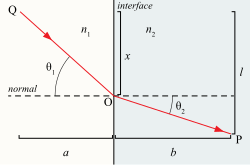
\includegraphics[width=0.33\textwidth]{speeds.png}
\caption{\label{fig:ray} A diagram of a light ray before and after crossing an interface between media with different indices of refraction.}
\end{figure}

\noindent
Consider a light ray $Q$ in a medium with index $n_1$ entering another medium at the origin $O$, and becoming a new ray $P$ (see Fig. \ref{fig:ray}).  $Q$ starts a vertical distance $x$ above $O$, and travels a total vertical distance of $l$.  $Q$ starts a horizontal distance $a$ from $O$, and travels a horizontal distance $b$ after $O$.  From the Pythagorean Theorem, the total distance traveled is

\begin{align}
\Delta r & & &= QO +OP \\
\Delta r & & &= \sqrt{a^2+x^2} + \sqrt{b^2 + (l-x)^2}
\end{align}

\textbf{Fermat's Principle} states that light takes the least possible time to travel from point to point.  From $\Delta r$, and the speeds of light $v_1$ and $v_2$ in the first and second medium, we can work out the time $T$ that elapses as the light travels from $Q$ to $P$:

\begin{align}
T & & &= QO/v_1 + OP/v_2 \\
T & & &= \frac{\sqrt{a^2+x^2}}{v_1} + \frac{\sqrt{b^2 + (l-x)^2}}{v_2} \\
T & & &= \frac{n_1\sqrt{a^2+x^2}}{c} + \frac{n_2\sqrt{b^2 + (l-x)^2}}{c} \label{eq:T}
\end{align}

We want to find the \textit{minimum} time $T$ to traverse $QO + OP$, and this restricts the value of $x$, which in turn restricts the relationship between $\theta_1$ and $\theta_2$.  The \textit{change} in $T$ with respect to $x$ can be calculated with the derivative\footnote{Do not worry if you are unfamiliar with differentiation.  This step is meant to illustrate how we relate the Law of Refraction to broader physical principles.} $dT/dx$.

\begin{equation}
\frac{dT}{dx} = \left(\frac{n_1}{c}\right) \frac{x}{\sqrt{a^2+x^2}} + \left(\frac{n_2}{c}\right) \frac{-(l-x)}{\sqrt{b^2 + (l-x)^2}}
\end{equation}

To \textit{minimize} $T$, we find the value of $x$ that makes \textit{the change in $T$} equal to zero.  Setting $dT/dx = 0$, we find

\begin{equation}
n_1 \frac{x}{\sqrt{a^2+x^2}} = n_2 \frac{(l-x)}{\sqrt{b^2 + (l-x)^2}}
\end{equation}

Notice that the ratio on the left side is $\sin\theta_1$, and the ratio on the right side is $\sin\theta_2$ (see Fig. \ref{fig:ray}).  Thus, we find

\begin{equation}
n_1 \sin\theta_1 = n_2 \sin\theta_2 \label{eq:sn2}
\end{equation} \\

\section{Experimental Setup}

\begin{figure}[ht]
\centering
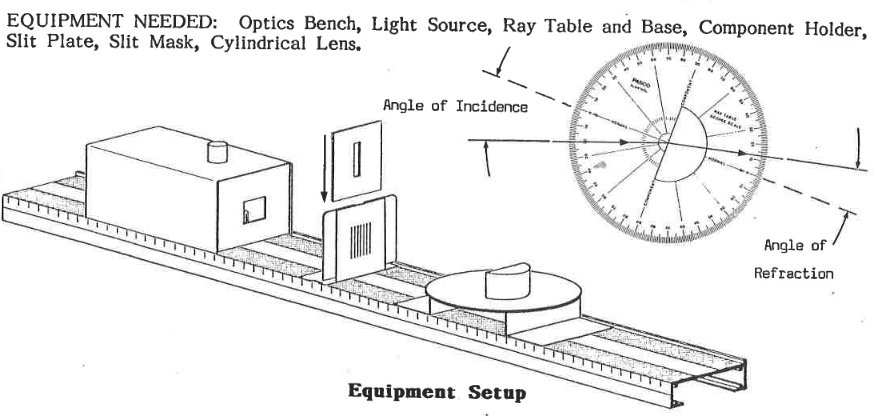
\includegraphics[width=0.49\textwidth]{equip.png}
\caption{\label{fig:equip} A diagram of the equipment arrangement.}
\end{figure}

\noindent
The procedure depicted in Fig. \ref{fig:equip} should produce results that verify Eq. \ref{eq:sn2} with $n_1 = 1.0$ for air.  Check that you have the following items at your table:

\begin{itemize}
\item Optics bench
\item Light source
\item Ray table and magnetic ray table base
\item Magnetic component holder
\item Slit plate and slit mask, magnetic
\item Cylindrical lens
\end{itemize}

Set the optics bench on the table with the magnetic ray table base in the center.  The ray table base is the magnetic base that is slanted on top.  The set the circular ray table on top of the base, with the degree markings visible.  You should also see markings for the \textit{normal} direction.  Align \textit{normal} with the direction of the optics bench.  Place the light source on the optics bench, facing the ray table.  The ray table should be slanted \textit{toward} the light source, so rays will be projected onto the degree markings.  Place the magnetic component holder between the ray table and light source.  The component holder should be as close to the ray table as possible without interfering with its rotation.  Check that the ray table can rotate freely.  Attach the slit mask on the component holder on the same side as the light source.  Attach the slit plate on the component holder on the side of the ray table.

Place the cylindrical lens in the center of the ray table with the flat side facing the light source and component holder.  The flat side of the cylindrical lens should align with a straight line on the ray table.  The normal direction on the ray table should be orthogonal to the flat side of the cylindrical lens.  The curved side of the lens has the cylindrical shape so that rays will not change direction as they leave the acrylic material of the lens.  If we zoom in to the point $R$ where the ray is leaving the cylindrical lens, the interrface at $R$ approaches a flat surface.  This is true regardless of the angle of incidence, and is true of any circle.  Thus, the ray will only change direction once, when it crosses from air into the lens via the flat side facing the light source.

\section{Data and Error Analysis}

\noindent
Activate the light source.  The light should pass through be emitted through the slits as a ray-like source with vertical extent.  The ray should project onto the ray table along the normal direction, marked with 0 degrees.  The ray should exit the cylindrical lens, and continue along the normal direction marked with 0 degrees.  If there is a slight misalignment, make a small adjustment using the knob on top of the light source.  The knob rotates the slight source by a few degrees, which helps ensure that 0 degrees into the lens corresponds to 0 degrees coming out of the lens.

As you rotate the ray table, add $\theta_2$ data to Tab. \ref{tab:data}.  We have set 0 degrees in to correspond to 0 degrees out, so we do not need to measure this.  Use Eq. \ref{eq:sn2} to calculate $n_2$.  The fact that the observed $n_2$ value is constant shows that Eq. \ref{eq:sn2} holds.

\begin{table}[ht]
\footnotesize
\centering
\begin{tabular}{| c | c | c | c |}
\hline
\textbf{$\theta_1$} [deg] & \textbf{$\theta_2$} [deg] & \textbf{$n_2 = \sin\theta_2/\sin\theta_1$} & \textbf{$\sigma_{n,2}$} \\ \hline
5 & & & \\ \hline
10 & & & \\ \hline
15 & & & \\ \hline
20 & & & \\ \hline
25 & & & \\ \hline
30 & & & \\ \hline
35 & & & \\ \hline
40 & & & \\ \hline
45 & & & \\ \hline
50 & & & \\ \hline
55 & & & \\ \hline
60 & & & \\ \hline
65 & & & \\ \hline
70 & & & \\ \hline
75 & & & \\ \hline \hline
\textbf{Average:} & --- & & \\ \hline
\end{tabular}
\caption{\label{tab:data} Perform the necessary measurements to complete this table.}
\end{table}

The error propagation formula for $n_2$ is

\begin{equation}
\frac{\sigma_{n,2}}{n_2} = \sqrt{\frac{\sigma_{\theta,1}^2}{\tan^2\theta_1} + \frac{\sigma_{\theta,2}^2}{\tan^2\theta_2}} \label{eq:err}
\end{equation}

Using Excel or Google sheets at your table, compute the error in $n_2$ using Eq. \ref{eq:err}.  The values for $\sigma_{\theta,1}$ and $\sigma_{\theta,2}$ are your decision based on the precision you perceive on the ray table.  Typical values are between 0.5 to 1.5 degrees, driven by the thickness of the light ray relative to the degree markings.

\section{Graphing the Data}

Did we just \textit{assume} Eq. \ref{eq:sn2} to be true, and then compute $n_2$ values based on this assumption?  If Eq. \ref{eq:sn2} does not hold, then our $n_2$ values would not be clustered tightly around the true constant value.  As a check, try graphing $\sin\theta_1$ versus $\sin\theta_2$.  The slope should be $n_2$, consistent with your value in Tab. \ref{tab:data}.  \textbf{Include a drawn version of your graph below.}

\end{document}